\section{Durchführung}
In diesem Versuch sollen die Bestandteile eines Würfels, welcher aus $27$ Elementarwürfeln mit einer Kantenlänge von 1 cm besteht, bestimmt werden.
Der zu Verfügung gestellte $\gamma$-Strahler ist $\ce{^{137}Cs}$, mit einem Peak $E_{\gamma} = \SI{661.7}{\k \eV}$.
Die Auswertung des Detektors erfolgt durch ein Computerprogramm, mit welchen auch die Daten ausgelesen werden können.
Die Messdauer für jede Messung wird auf $\SI{240}{\second}$ eingestellt.
Zunächst wird eine Leermessung durchgeführt, um eine Zuordnung des $\gamma$-Peaks zu ermöglichen. 
Außerdem wird auch ein vollständiges $\gamma$-Spektrum aufgenommen und dokumentiert.
Daraufhin wird ein leeres Aluminiumgehäuse, in welchem sich die Würfel befinden, vermessen.
Anschließend wird der Würfel 3 vermessen, welcher nur aus einem Material besteht. 
Hierfür werden insgesamt vier Strahlengänge gewählt und die Anzahl der $\gamma$-Teilchen mithilfe des Programms ausgelesen.
Zuletzt wird der Würfel 4 vermessen, welcher aus zwei verschiedenen Materialen besteht. 
Hierfür werden insgesamt zwölf Strahlengänge untersucht und erneut die Teilchenanzahl mithilfe des Detektors ausgelesen. 
In Abbildung \ref{fig:tikz1} sind die untersuchten Projektionen dargestellt. 
\begin{figure}
    \centering
    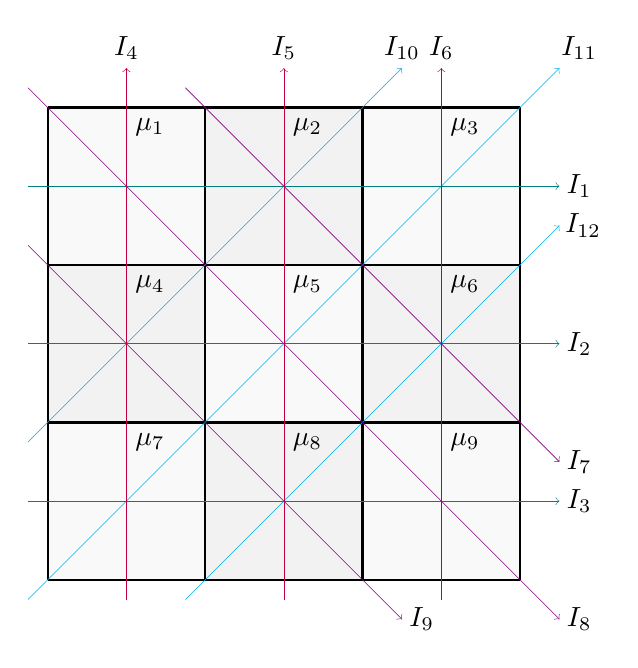
\begin{tikzpicture}

        \node[fill=gray!5, minimum size=2cm] at (1,1) {};
        \node[fill=gray!5, minimum size=2cm] at (1,5) {};
        \node[fill=gray!5, minimum size=2cm] at (5,1) {};
        \node[fill=gray!5, minimum size=2cm] at (5,5) {};
        \node[fill=gray!5, minimum size=2cm] at (3,3) {};

        \node[fill=gray!10, minimum size=2cm] at (3,1) {};
        \node[fill=gray!10, minimum size=2cm] at (1,3) {};
        \node[fill=gray!10, minimum size=2cm] at (5,3) {};
        \node[fill=gray!10, minimum size=2cm] at (3,5) {};

        \draw[step = 2cm, thick] (0,0) grid +(6,6);

        \draw[->][cyan, very thin] (-0.25,-0.25)--(6.5,6.5);
        \node at (6.75,6.75) {$I_{11}$};
        \draw[->][cyan, very thin] (-0.25,1.75)--(4.5,6.5);
        \node at (4.5,6.75) {$I_{10}$};
        \draw[->][cyan, very thin] (1.75,-0.25)--(6.5,4.5);
        \node at (6.8,4.5) {$I_{12}$};
        \draw[->][violet, very thin] (1.75,6.25)--(6.5,1.5);
        \node at (6.75,1.5) {$I_{7}$};
        \draw[->][violet, very thin] (-0.25,6.25)--(6.5,-0.5);
        \node at (6.75,-0.5) {$I_{8}$};
        \draw[->][violet, very thin] (-0.25,4.25)--(4.5,-0.5);
        \node at (4.75,-0.5) {$I_{9}$};
        \draw[->][teal, very thin] (-0.25,5)--(6.5,5);
        \node at (6.75,5) {$I_{1}$};
        \draw[->][teal, very thin] (-0.25,3)--(6.5,3);
        \node at (6.75,3) {$I_{2}$};
        \draw[->][teal, very thin] (-0.25,1)--(6.5,1);
        \node at (6.75,1) {$I_{3}$};
        \draw[->][purple, very thin] (1,-0.25)--(1,6.5);
        \node at (1,6.75) {$I_{4}$};
        \draw[->][purple, very thin] (3,-0.25)--(3,6.5);
        \node at (3,6.75) {$I_{5}$};
        \draw[->][purple, very thin] (5,-0.25)--(5,6.5);
        \node at (5,6.75) {$I_{6}$};
        \node at (1.3,1.75) {$\symbf{\mu_7}$};
        \node at (1.3,3.75) {$\symbf{\mu_4}$};
        \node at (1.3,5.75) {$\symbf{\mu_1}$};
        \node at (3.3,1.75) {$\symbf{\mu_8}$};
        \node at (3.3,3.75) {$\symbf{\mu_5}$};
        \node at (3.3,5.75) {$\symbf{\mu_2}$};
        \node at (5.3,1.75) {$\symbf{\mu_9}$};
        \node at (5.3,3.75) {$\symbf{\mu_6}$};
        \node at (5.3,5.75) {$\symbf{\mu_3}$};
    \end{tikzpicture}
    \caption{Die einzelen Projektionsrichtungen die im Experiment zur Bestimmung der Absorptionskoeffizienten der neun Elementarwürfel
    untersucht werden. Erstellt mit der \LaTeX-Erweiterung TikZ \cite{tantau:2013a}.}
    \label{fig:tikz1}
\end{figure}
Mit dieser Wahl der Projektionen hat die Matrix $D$ die Form 
\begin{equation*}
    D = \begin{pmatrix*}[c]
        1 & 1 & 1 & 0 & 0 & 0 & 0 & 0 & 0 \\ %1
        0 & 0 & 0 & 1 & 1 & 1 & 0 & 0 & 0 \\ %2
        0 & 0 & 0 & 0 & 0 & 0 & 1 & 1 & 1 \\ %3
        1 & 0 & 0 & 1 & 0 & 0 & 1 & 0 & 0 \\ %4
        0 & 1 & 0 & 0 & 1 & 0 & 0 & 1 & 0 \\ %5
        0 & 0 & 1 & 0 & 0 & 1 & 0 & 0 & 1 \\ %6
        0 & \sqrt{2} & 0 & 0 & 0 & \sqrt{2} & 0 & 0 & 0 \\ %7
        \sqrt{2} & 0 & 0 & 0 & \sqrt{2} & 0 & 0 & 0 & \sqrt{2} \\ %8
        0 & 0 & 0 & \sqrt{2} & 0 & 0 & 0 & \sqrt{2} & 0 \\ %9
        0 & \sqrt{2} & 0 & \sqrt{2} & 0 & 0 & 0 & 0 & 0 \\ %10
        0 & 0 & \sqrt{2} & 0 & \sqrt{2} & 0 & \sqrt{2} & 0 & 0 \\ %11
        0 & 0 & 0 & 0 & 0 & \sqrt{2} & 0 & \sqrt{2} & 0 \\ %12
    \end{pmatrix*} \, .
\end{equation*}
